
\section{Use case: broadcasting messages}
\label{sec:usecase}


%In this section, we evaluate the benefits that \SPRAY can bring to
%protocols built on top of it. Using the example of a broadcast
%mechanism, we expect \SPRAY to keep a stable delivery rate on messages
%while supporting network size variations. Then, 

In this section, we highlight how protocols built on top of \SPRAY can
benefit from its adaptiveness. We focus on broadcasting
messages. Firstly, we consider the case of video streaming using a
three-phase gossip protocol~\cite{FlightPath,Frey09DSN,monod:THESIS}.
Using \SPRAY, we expect a stable message-delivery rate even when the
size of the network fluctuates. Using \CYCLON, we expect degraded
performance when the size of the network is larger than expected at
configuration time. Secondly, we use the case of \emph{gossiping} in
decentralized real-time collaborative editing. Using \SPRAY, we expect
the generated traffic to scale logarithmically with respect to the
size of the network.

The first experiment runs on the \PEERSIM simulator~\cite{montresor2009peersim}
and the code is available on the Github
platform\footnote{\url{https://github.com/justayak/peersim-spray}}. The second
experiment is a simulation involving up to 600 interconnected Web browsers on
the Grid'5000 testbed. The code is available on the Github
platform\footnote{\url{https://github.com/Chat-Wane/CRATE}}.

\subsection{Streaming}

Live video streaming has grown in importance over recent years and
companies offering peer-to-peer streaming gather large numbers of
viewers. For example,
HiveStreaming\footnote{\url{https://www.hivestreaming.com/}} declared
having a customer network of 400k peers~\cite{smoothcache2}. The
uploading bitrate required to serve such a large number of users would
lead to huge operational costs, which can instead be saved through
direct peer-to-peer exchanges.

\subsubsection{Operation}
A number of existing
systems~\cite{Frey09Middleware,monod:THESIS,Zhang07Understanding} use
some variant of gossip to achieve effective stream dissemination in
the presence of churn. In the following, we consider the three-phase
variant adopted
by~\cite{Frey09DSN,FlightPath,monod:THESIS,Zhang07Understanding}. Nodes
gossip advertisement messages for available packets to \emph{fanout}
other nodes, which then pull the packets they need.
Algorithm~\ref{algo:threephase} details the operation of this protocol.
First, with a time interval of $\delta$ ($200ms$
in~\cite{Frey09DSN,Frey09Middleware}), each peer advertises the packets
it can serve to $f$ (fanout) neighbors. Second, a peer receiving such
an advertisement requests the packets it needs. Third, the advertising
peer sends the requested packets.

In their analysis of this three-phase model, the authors
of~\cite{Frey09DSN} observed that, in bandwidth-constrained scenarios,
peers should vary their communication partners as often as possible in
order to equalize everyone's contribution. There are two ways to
achieve this in a large scale setting:
\begin{inparaenum}[(i)]
\item \label{enum:refreshing} refreshing the view of the peer-sampling protocol
  (e.g. \CYCLON, or \SPRAY) before sending each advertisement packet, or
\item \label{enum:larger} using a view that is much larger than the gossip
  fanout and refreshing it less often.
\end{inparaenum}
Due to the relatively small size of view-exchange messages, solution
(\ref{enum:larger}) achieves the best trade-off, while solution
(\ref{enum:refreshing}) is extremely impractical and waste a significant
amount of bandwidth just for packet headers---\cite{Frey09DSN,Frey09Middleware}
have each node send $5$ advertisement packets per second.

For this reason, \cite{frey:hal-01479885} follows solution (\ref{enum:larger})
and sets the fanout to $\ln(N)+c$ (according to theory~\cite{PRD}), $N$ being the
number of participating peers, and $c$ being a positive constant.

\begin{algorithm}[h]
  
\small
\algrenewcommand{\algorithmiccomment}[1]{\hskip2em$\rhd$ #1}

\newcommand{\comm}[1]{$\rhd$ #1}

\newcommand{\LINEFOR}[2]{%
  \algorithmicfor\ {#1}\ \algorithmicdo\ {#2} %
  }

\newcommand{\LINEIFTHEN}[2]{%
  \algorithmicif\ {#1}\ \algorithmicthen\ {#2} %
  }

\newcommand{\INDSTATE}[1][1]{\State\hspace{\algorithmicindent}}

\algblockdefx[initially]{initially}{endInitially}
[0] {\textbf{INITIALLY:}} 

\algblockdefx[act]{act}{endAct}
[0] {\textbf{ACTIVE THREAD:}}

\algsetblockdefx[pas]{pas}{endPas}
{65535}{}
[0] {\textbf{PASSIVE THREAD:}}


\begin{algorithmic}[1]
  \Statex
  \initially
  \State $B$ \hfill \comm{buffer of packets}
  \State $b$ \hfill \comm{number of advertised packets}
  \State $f$ \hfill \comm{fanout $f \leq |P|$}
  \endInitially
  
  \act
  \Function{advertisementLoop}{$(\,)$} \hfill \comm{every $\delta$ time} 
  \State \textbf{let} $advertiseTo \leftarrow getPeers(P,\,f)$; \hfill \comm{$f$ distinct random peers from $P$}
  \State \textbf{let} $advertisement \leftarrow getIdentifiers(B,\,b)$; \hfill \comm{$b$ distinct random packet Ids}
  \State \LINEFOR{\textbf{each} $q \in advertiseTo$}{$sendTo(q,\, 'advertisement',\, advertisement)$;}
  \EndFunction
  \endAct

  \pas
  \Function{onAdvertisement}{$o,\, ads$} \hfill \comm{$o: advertiser$}
  \For {\textbf{each} $(id \in ads)$}
  \State \LINEIFTHEN{$id \not\in B$}{$sendTo(o,\, 'request',\, id)$;}
  \EndFor  
  \EndFunction
  
  \State
  \Function{onRequest}{$o,\, id$} \hfill \comm{$o: requester$}
  \State \textbf{let} $packet \leftarrow getMessage(B,\,id)$; \hfill \comm{get the requested packet from the buffer}
  \State $sendTo(o, \, packet)$; \hfill \comm{finally send the packet}
  \EndFunction

\end{algorithmic}

  \caption{\label{algo:threephase}Three-phase gossip.}
\end{algorithm}



\subsubsection{Experimentation}

\begin{asparadesc}
\item [Objective:] To show how broadcast protocols can benefit from
  an adaptive random peer sampling protocol.
\item [Description:] 
  % Broadcast protocols extensively use the partial views provided by random peer
  % sampling protocols to efficiently disseminate messages to all the network. A
  % broadcasting peer chooses some neighbors from its partial view to whom it
  % sends the message. Each peer receiving such a message broadcasts it once, in
  % an identical way. The message transitively reaches all members. The number of
  % chosen neighbors is called the \emph{fanout}. Since several applications need
  % to broadcast messages more frequently than they can shuffle their neighbors,
  % broadcast protocols tend to use view sizes that are much larger than the
  % broadcast fanout~\cite{Frey09Middleware}. This allows the peer-sampling
  % protocol to provide the application with fresh peers at each broadcast round
  % without having to wait for the network's mixing
  % time~\cite{jelasity2007gossip}. 
  In this experiment, we reproduce the first gossip phase of the
  protocol in~\cite{Frey09DSN,frey:hal-01479885,monod:THESIS} and model an
  application that streams live content to $100$ peers.
  % : a user streaming the live video of a local sport event.
  We configure \CYCLON's partial view to $6$ times the threshold
  fanout required for $100$ nodes ($6 \ln(100) \approx 6 \cdot 5 =
  30$, analogously to~\cite{frey:hal-01479885}), and consider two configurations
  for the broadcast fanout $\ln(100)+1 \approx 6 $ and $\ln(100)+3
  \approx 8$, which provide high reliability with $100$
  nodes. Similarly, we configure \SPRAY to have partial views size
  equal to $6 \cdot \ln(|V^t|)$---instead of adding only 1 arc
  targeting its contact (see Section \ref{subsec:joining}), the
  newcomer adds 6 arcs---and sets the fanout to one sixth of the view
  size plus $1$ or $3$. This gives both protocols the same
  configuration for $100$ peers.  We then consider network sizes
  growing from $100$ to $2000$ peers, and measure the ratio of fully
  delivered messages to 1k sent messages, i.e., we evaluate the
  fraction of all messages that reach all the members of the network.

\begin{figure}
  \begin{center}
    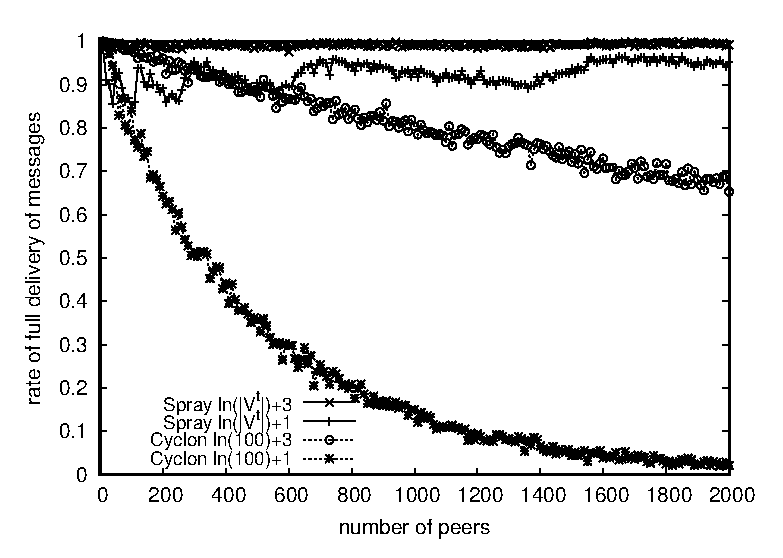
\includegraphics[width=\SCALE\textwidth]{img/hardrate.eps}
    \caption{\label{fig:hardrate}Ratio of messages fully delivered.}
  \end{center}
\end{figure}

\item [Results:] Figure~\ref{fig:hardrate} shows the results of this
  experiment. First, we observe that the ratio of fully delivered
  messages using \CYCLON suffers from a steady decrease. The highest
  fanout leads to better results. In contrast, \SPRAY remains stable
  despite the presence of small jumps. A fanout set to $\ln(|V^t|)+1$
  gives a full delivery ratio above 90\%. A fanout set to
  $\ln(|V^t|)+3$ is very close to 100\%. Overall, the broadcast
  mechanism benefits from the adaptive nature of \SPRAY's partial
  view, which allows it to scale according to the size of the network.
\item [Reasons:] To ensure a fair use of the bandwidth contributed by
  peers, we configure the view size to be larger than the fanout. This
  allows stream packets in three-phase gossip to follow ``almost''
  random subtrees of the complete overlay. But it also leads the first
  gossip phase to require a fanout of at least $\ln(N)+c$~\cite{PRD},
  as the random sub-graphs of the overlay grafted in the first phase
  may fail to reach all nodes if the fanout is too low. In our case,
  the broadcast protocol built on top of \CYCLON has a constant fanout
  set for a specific network size. As long as the network is smaller
  than this value, the full delivery ratio stays high. However, it
  quickly decreases with larger network sizes.  \SPRAY instead allows
  the application fanout to follow the growth of the partial view
  size, which scales logarithmically compared to the network
  size. This allows the streaming application to adapt to changes in
  the size of the network. As a result, the full delivery ratio
  provided by the broadcast mechanism on top of \SPRAY remains
  stable. Since the values manipulated by peers---partial view size
  and fanout---are integers, the measurements make small jumps when a
  rounded value increases enough to be incremented.
\end{asparadesc}

\ \\

\begin{asparadesc}
\item [Objective:] To show how the full delivery ratio behaves during a buzz,
  i.e., a sudden massive increasing of network size shortly followed by
  departures.
\item [Description:] We configure \SPRAY and \CYCLON like in the
  previous experiment. For \CYCLON, we use a partial view size of 30
  and two broadcast fanout values: $\ln(100)+1$ and $\ln(100)+3$. For
  \SPRAY, we use a dynamic view of $6 \cdot \ln(|V^t|)$ and broadcast
  fanout values of $\ln(|V^t|)+1$ and $\ln(|V^t|)+3$. The simulation
  starts with 100 peers. The network quickly reaches 10k peers during
  the popularity burst. Then the network size decreases to 3k
  members. In this experiment, we measure the full delivery ratio over
  each group of 100 consecutive messages.

\begin{figure}
  \begin{center}
    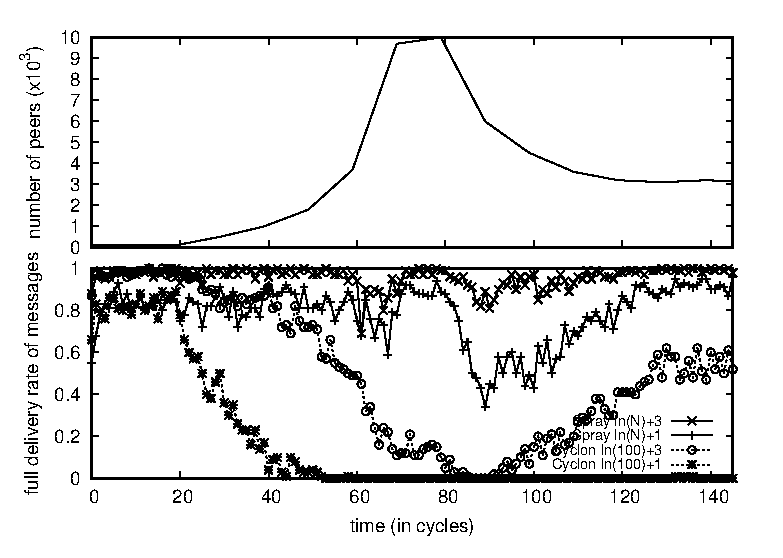
\includegraphics[width=\SCALE\textwidth]{img/peak.eps}
    \caption{\label{fig:peak}Full message delivery ratio during a buzz.}
  \end{center}
\end{figure}

\item [Results:] Figure~\ref{fig:peak} shows the results of this
  experiment. The top part of the figure shows the evolution of the
  network size over time. The bottom figure shows the full delivery
  ratio over time. Like in the previous experiment,
  Figure~\ref{fig:peak} shows that using \CYCLON and a predefined
  fanout works well until the network size reaches an unexpected
  size. During the peak, the delivery ratio falls quickly. Conversely,
  the broadcast mechanism built on top of \SPRAY automatically adapts
  the fanout to the size of the network. Thus, it does not experience
  performance losses while a large number of nodes suddenly join, even
  though we observe a decrease in delivery ratio during the departures
  of peers, in particular with a fanout of $\ln(|V|)+1$. This
  demonstrates that, in the context of three-phase gossip, \SPRAY
  makes broadcast more resilient to quick membership changes.
\item [Reasons:] The fanout of configurations involving \CYCLON is
  constant. When the number of peers in the network exceeds the
  expectations, the delivery ratio quickly degenerates. Concerning
  \SPRAY, the fanout follows the evolution of the network thanks to
  adaptive partial views. Both \SPRAY and \CYCLON detect departing
  nodes during the shuffling phase. The associated delay leads to the
  use of some stale arcs from partial views, which explains the
  temporary decrease in delivery ratio during the shrinking
  phase. Since both \CYCLON and \SPRAY clean their partial views over
  time, the delivery ratio recovers its expected value.
\end{asparadesc}


\subsection{Real-time editing}

%In order to demonstrate the performance of \SPRAY with a real scenario, we
%introduce 
\CRATE is a real-time editor that allows authors to write anytime and
anywhere, whatever the number of participants, without any third
party~\cite{nedelec2016crate}. Compared to trending Cloud-based
editors such as Google Docs, it alleviates privacy, scalability, and
single-point-of-failure issues while remaining easy to use.  It can be
used for small groups but also during events such as massive online
lectures, TV shows, or conferences that gather larger groups. For
instance, online lecture sessions reach thousands of
students. Transitions between small groups and large groups is
supported transparently thanks to \SPRAY. Distributed real-time
editing is a pertinent context for \SPRAY for group sizes differ
depending on the document, and change quickly over time.

\CRATE builds a network of browsers where each browser is able to
communicate with a logarithmically scaling number of browsers compared
to the global network size. Each change performed on documents
transits through neighbors and reaches all members in a scalable
way~\cite{birman1999bimodal}. Unlike the
state-of-the-art~\cite{tolgyeski2009adaptive,voulgaris2005cyclon},
\SPRAY allows the diffusion cost to adapt to the network size without
any probing mechanism or any central authority.  Without \SPRAY,
developers would have to overestimate the parameters of peer-sampling
protocols to get a system that behaves well for large as well as for
small networks. This would increase the cost of maintaining
connections alive (e.g. in a WebRTC context) and more importantly the
cost of application protocols (e.g. broadcasting protocols).  \SPRAY,
on the other hand, ensures that small networks do not pay the price of
large networks without requiring the intervention of developers or
end users. 

\subsubsection{Operation}

To provide availability and responsiveness in documents, collaborative
editors consider multiple authors, each hosting a replica of their
shared document~\cite{saito2005optimistic}.  On updates, the local
replica is directly modified. Then, each update is propagated to all
the editing session where it is integrated. Strong eventual
consistency~\cite{bailis2013eventual} states that a system is correct
if and only if the replicas converge to an equivalent state when they
integrated the same updates. In other terms, the users read identical
documents.

\CRATE uses a distributed sequence data type~\cite{shapiro2011conflict} which
provides two commutative operations: the insertion and the removal of an
element. Commutativity allow users to avoid the difficult, time consuming, and
error-prone task of solving conflicts due to concurrent edits. However,
commutativity comes at the price of metadata attached to each character. These
metadata (referred to as \emph{identifiers}) are unique and immutable. The
structure representing an identifier is a list $[\ell_1.\ell_2\ldots\ell_k]$ the
size $k$ of which is determined during allocation. \CRATE uses an allocator
function~\cite{nedelec2013lseq} to keep these identifiers under acceptable
growth, i.e., a polylogarithmic upper bound on their space complexity compared
to the document size: $\mathcal{O}((\log |document|)^2)$.

% An identifier is a list $[\ell_1.\ell_2\ldots\ell_k]$ where $k$ is the
% identifier depth. A total order among identifiers allows retrieving the
% sequence of characters. To encode such total order, the structure uses a simple
% lexicographic order comparing
% \begin{inparaenum}[(i)]
% \item paths -- chosen by the allocator and the most important as it determines
%   the space complexity of the approach --
% \item globally unique identifiers -- required for uniqueness and necessary in
%   some concurrent cases.
% \end{inparaenum}
% We focus our description on paths.

% \begin{figure}
%   \centering
%   \begin{tikzpicture}[scale=1.1]

\newcommand\Y{-45}
\newcommand\ADDY{-8}

  \scriptsize
  \draw[dashed] (340pt,10pt) node[anchor=north west]{maximum arity}  -- (340pt,3*\Y pt);
  \draw[dashed] (390pt,0 pt)  --(330pt,0 pt);
  \draw[dashed] (390pt,\Y pt) -- (330pt,\Y pt);
  \draw[dashed] (390pt,2*\Y pt) -- (330pt,2*\Y pt);
  \draw[dashed] (390pt,3*\Y pt) -- (330pt,3*\Y pt);

  \draw (340pt,0.5*\Y pt)
  node[anchor=west, align=center]{$32$};
  \draw (340pt,1.5*\Y pt)
  node[anchor=west, align=center]{$64$};
  \draw (340pt,2.5*\Y pt)
  node[anchor=west, align=center]{$128$};

  \begin{scope}[shift={(90pt,0pt)}]
\begin{scope}[shift={(160pt,0pt)}]
  \draw[->,dashed](50pt,3*\Y + 10 pt)--node[anchor=north]{insertion order}
  (-50pt,3*\Y + 10 pt);
  %% node to node
  \scriptsize
  \draw[thick] (0pt,0pt) -- node[anchor=south east]{0} (-70pt,\Y pt);
  \draw[thick] (0pt,0pt) -- node[anchor=east]{1} (50pt, \Y pt); %% Y
  \draw[thick] (-70pt, \Y pt) -- node[anchor=north]{57} (30pt, 2 * \Y pt); %% T
  \draw[thick] (-70pt, \Y pt) -- node[anchor=north]{56} (10pt, 2 * \Y pt); %% R
  \draw[thick] (-70pt, \Y pt) -- node[anchor=north]{53}(-10pt, 2 * \Y pt);%% E
  \draw[thick] (-70pt, \Y pt) -- node[anchor=north]{48}(-30pt,2 * \Y pt); %% W
  \draw[thick] (-70pt, \Y pt) -- node[anchor=east]{44}(-50pt,2 * \Y pt); %% Q
  \draw[dashed, thick] (0pt,0pt) -- node[anchor=south west]{32} (70pt,\Y pt);

  %% node to element
  \draw[->] ( 50pt, \Y pt) -- ( 50pt, \ADDY + \Y pt); %% Y
  \draw[->] ( 30pt, 2* \Y pt) -- ( 30pt, \ADDY + 2 *\Y pt); %% T
  \draw[->] ( 10pt, 2 *\Y pt) -- ( 10pt, \ADDY + 2 *\Y pt); %% R
  \draw[->] (-10pt, 2 *\Y pt) -- (-10pt, \ADDY + 2 *\Y pt); %% E
  \draw[->] (-30pt, 2 *\Y pt) -- (-30pt, \ADDY + 2 *\Y pt); %% W
  \draw[->] (-50pt, 2 *\Y pt) -- (-50pt, \ADDY + 2 *\Y pt); %% Q

  %% element to desambiguator
  \draw[->,densely dashdotted]
  ( 50pt, \ADDY + \Y pt) -- ( 50pt,2.75*\ADDY+\Y pt); %% Y
  \draw[->,densely dashdotted]
  ( 30pt, \ADDY + 2* \Y pt) -- ( 30pt,2.75*\ADDY+ 2* \Y pt); %% T
  \draw[->,densely dashdotted]
  ( 10pt, \ADDY + 2* \Y pt) -- ( 10pt,2.75*\ADDY+ 2* \Y pt); %% R
  \draw[->,densely dashdotted]
  ( -10pt, \ADDY + 2 *\Y pt) -- (-10pt,2.75*\ADDY+ 2* \Y pt); %% E
  \draw[->,densely dashdotted]
  ( -30pt, \ADDY + 2 *\Y pt) -- (-30pt,2.75*\ADDY+ 2*\Y pt); %% W
  \draw[->,densely dashdotted]
  ( -50pt, \ADDY + 2* \Y pt) -- (-50pt,2.75*\ADDY+ 2*\Y pt); %% Q

  %% node
  \draw[fill=black] (0pt,0pt) circle (1pt); %% rooot
  \draw[fill=white] ( 50pt, \Y pt) circle (1pt); %% Y
  \draw[fill=white] (-70pt, \Y pt) circle (1pt); %% 0
  \draw[fill=white] ( 30 pt, 2 * \Y pt) circle (1pt); %% T
  \draw[fill=white] ( 10 pt, 2 * \Y pt) circle (1pt); %% R
  \draw[fill=white] (-10 pt, 2 * \Y pt) circle (1pt); %% E
  \draw[fill=white] (-30 pt, 2 * \Y pt) circle (1pt); %% W
  \draw[fill=white] (-50 pt, 2 * \Y pt) circle (1pt); %% Q
  \draw[fill=black] ( 70pt, \Y pt) circle (1pt);


  %% elements
  \draw[fill=white] ( 50pt, -4 + \ADDY + \Y pt)
  node{\textbf{Y}} +(-4pt,-4pt) rectangle +(4pt,4pt) ; %% Y
  \draw[fill=white] ( 30pt, -4 + \ADDY +  2 *\Y pt)
  node{\textbf{T}} +(-4pt,-4pt) rectangle +(4pt,4pt) ; %% T
  \draw[fill=white] ( 10pt, -4 + \ADDY +  2* \Y pt)
  node{\textbf{R}} +(-4pt,-4pt) rectangle +(4pt,4pt) ; %% R
  \draw[fill=white] (-10pt, -4 + \ADDY + 2 *\Y pt)
  node{\textbf{E}} +(-4pt,-4pt) rectangle +(4pt,4pt) ; %% E
  \draw[fill=white] (-30pt, -4 + \ADDY + 2 * \Y pt)
  node{\textbf{W}} +(-4pt,-4pt) rectangle +(4pt,4pt) ; %% W
  \draw[fill=white] (-50pt, -4 + \ADDY + 2 *\Y pt)
  node{\textbf{Q}} +(-4pt,-4pt) rectangle +(4pt,4pt) ; %% Q

  %% desambiguator
  \draw[fill=gray!20]( 50pt, -2.5 + 2.75 * \ADDY + \Y pt)
  +(-2.5pt,-2.5pt) rectangle +(2.5pt,2.5pt);
  \draw[fill=gray!20]( 30pt, -2.5 + 2.75 * \ADDY +2 *\Y pt)
  +(-2.5pt,-2.5pt) rectangle +(2.5pt,2.5pt);
  \draw[fill=gray!20]( 10pt, -2.5 + 2.75 * \ADDY +2*\Y pt)
  +(-2.5pt,-2.5pt) rectangle +(2.5pt,2.5pt);
  \draw[fill=gray!20](-10pt, -2.5 + 2.75 * \ADDY +2*\Y pt )
  +(-2.5pt,-2.5pt) rectangle +(2.5pt,2.5pt);
  \draw[fill=gray!20](-30pt, -2.5 + 2.75 * \ADDY +2*\Y pt)
  +(-2.5pt,-2.5pt) rectangle +(2.5pt,2.5pt);
  \draw[fill=gray!20](-50pt, -2.5 + 2.75 * \ADDY +2*\Y pt) 
  +(-2.5pt,-2.5pt) rectangle +(2.5pt,2.5pt);

\end{scope}
\end{scope}

\end{tikzpicture}

%   \caption{\label{fig:lseqexample}\LSEQ data structure representing QWERTY.}
% \end{figure}

% When an insert operation is performed at a specific index in the document
% through the graphical user interface, the event is forwarded to the distributed
% data structure which translates it into \emph{allocate an identifier between the
%   identifiers adjacent to the targeted position}.  Figure~\ref{fig:lseqexample}
% shows the data structure resulting of the following editing sequence: insert 'Y'
% at 0, insert 'T' at 0, insert 'R' at 0, \ldots, insert 'Q' at 0. First, we
% observe that \LSEQ factorizes identifiers under an exponential tree
% representation. Indeed, as the depth of the tree grows, the number of potential
% children doubles. When the first insertion of Character 'Y' arrives, it
% allocates a path between the virtual adjacent identifiers paths [0] and
% [32]. Here it chooses the path [1] which is unfortunate since other insertions
% arrive preceding this character. Since there is no room for more paths at the
% first level between the virtual beginning boundary and the path of Character Y,
% the depth of the tree must grow. The new identifier is allocated between [0.0]
% and [0.64] which result in the path [0.57], etc. At the end, all identifiers are
% comparable and the resulting sequence of characters is 'QWERTY'.

An editor sends each pair of identifier and character to all members of the
editing session. For this purpose, \CRATE uses a very simple broadcast protocol
built on top of \SPRAY following the principles of epidemic dissemination (also
known as gossiping)~\cite{demers1987epidemic}. Such mechanisms make extensive
use of partial views to efficiently disseminate messages.

% Compared to Google Docs, \CRATE is decentralized and preserves
% privacy. It also supports any number of participants where Google Docs
% allows only the first fifty users to edit in real-time. Additional
% users have their rights limited to document reading.

% \subsection{Epidemic dissemination}
% \label{subsec:gossiping}

% Epidemic dissemination~\cite{birman1999bimodal,demers1987epidemic} (or
% gossiping) relies on the membership protocol to propagate messages in a scalable
% way to all members (broadcast).

\begin{algorithm}[h]
  
\small
\algrenewcommand{\algorithmiccomment}[1]{\hskip2em$\rhd$ #1}

\newcommand{\comment}[1]{$\rhd$ #1}

\newcommand{\LINEFOR}[2]{%
  \algorithmicfor\ {#1}\ \algorithmicdo\ {#2} %
  }

\newcommand{\LINEIFTHEN}[2]{%
  \algorithmicif\ {#1}\ \algorithmicthen\ {#2} %
  }

\newcommand{\INDSTATE}[1][1]{\State\hspace{\algorithmicindent}}

\begin{algorithmic}[1]
  \Function{broadcast}{$m$} \hfill \comment{$m: message$}
    \State \LINEFOR{\textbf{each} $\langle q,\,\_\, \rangle \in\mathcal{P}$}
    {$sendTo(q,\, 'broadcast',\, m)$;}
    \EndFunction
    \Statex
  \Function{receiveBroadcast}{$m$} \hfill \comment{$m: message$}
  \If {$\neg alreadyReceived(m)$}
  \State $deliver(m)$;
  \State $broadcast(m)$;
  \EndIf
  \EndFunction
  
\end{algorithmic}

  \caption{\label{algo:gossiping}gossip.}
\end{algorithm}

Algorithm~\ref{algo:gossiping} shows the instructions of this protocol. When a
peer emits a message, it sends it to its neighborhood. Each peer receiving such
messages for the first time forwards it to its neighborhood too. Messages
transitively reach all network members.

Since the gossiping algorithm depends of the neighborhood provided by \SPRAY,
and since the latter grows logarithmically compared to the network size, the
communication complexity of an application is upper-bounded by
$\mathcal{O}(m \ln |V^t|)$, where $m$ is the space complexity of a
message. Since \CRATE's identifiers are sublinearly upper-bounded compared to
the document size, \CRATE scales well.


\subsubsection{Experimentation}
\label{subsec:experiments2}

We highlight the improvements brought to protocols built on top of \SPRAY on a
real-life use case about decentralized collaborative editing in Web browsers.

% These experiments run on the Grid'5000 testbed and involve up to 600 browsers
% simultaneously writing a document. Using \SPRAY, we expect a traffic
% logarithmically scaling compared to the network size, along with a
% polylogarithmic growth brought by the real-time editor itself.

%%\vspace{-7pt}
%%\paragraph{CRATE on network of browsers}

\begin{asparadesc}
\item [Objective:] To show that the traffic generated by \SPRAY stays low
  compared to the traffic generated by broadcasting. To show the influence of
  \SPRAY's adaptiveness over the traffic generated by decentralized editors
  running on a network of browsers.
\item [Description:] Experiments run on Grid'5000 where machines host 5 browsers
  each. Browsers open \CRATE and connect to an editing session through a
  signaling server.  Runs comprise from 101 browsers to 601 browsers with 100
  browsers increments, i.e., 6 different runs.  The first editor creates the
  editing session which is progressively joined by the other writers (1 joiner
  per 5 seconds). Each member starts sharing the access to the editing session
  as soon as it joins it. Outsiders join the network through one of them chosen
  at random. Once all peers have joined the editing session, the document
  editing starts. The insertion rate is 100 insertions per second uniformly
  distributed among peers. Each experiment runs during 8 hours of which 7 hours
  are dedicated to editing. The document size reaches millions of characters.

% \begin{figure}
%   \centering
%   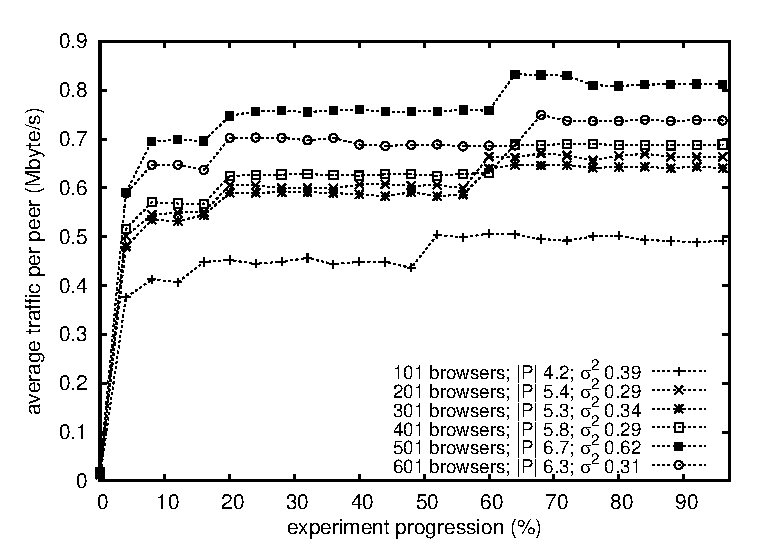
\includegraphics[width=\SCALE\textwidth]{img/traffic.eps}
%   \caption{\label{fig:traffic}Average traffic per second.}
% \end{figure}

\begin{figure*}
\centering
\subfloat[Figure A]
[\label{fig:warmup}Warmup time: peers join the session. Only \SPRAY generates
the outgoing traffic.]
{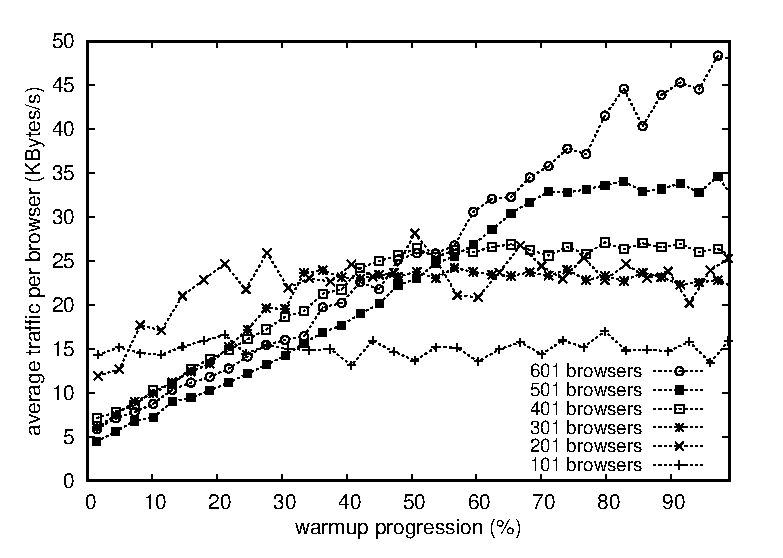
\includegraphics[width=0.8\textwidth]{img/warmup.eps}}

\subfloat[Figure B]
[\label{fig:traffic}Editing time: peers write a document. Both \SPRAY 
and \CRATE generate the outgoing traffic.]
{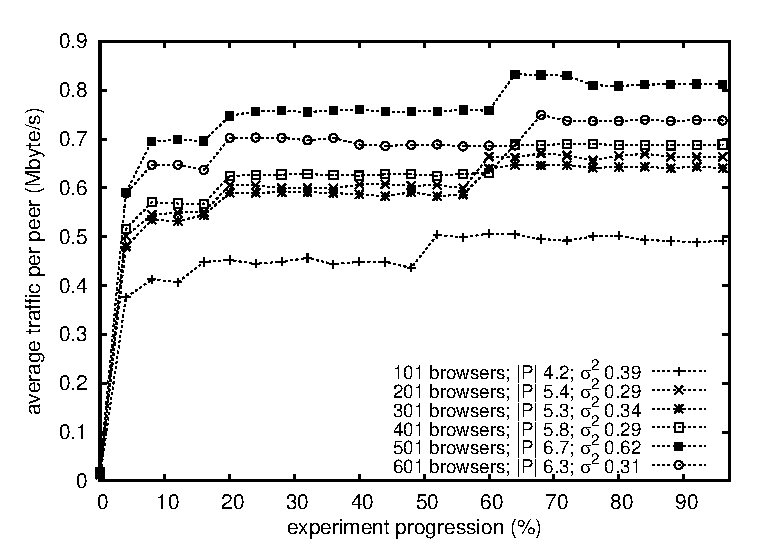
\includegraphics[width=0.8\textwidth]{img/traffic.eps}}
\caption{Average traffic per second generated by a real application.}
\end{figure*}


\item [Results:] Figure~\ref{fig:warmup} and Figure~\ref{fig:traffic} show the
  average traffic per second generated by members involved in collaborative
  editing. The x-axis denote the time progression of the warmup and the
  experiment in percentage over 45 minutes and 7 hours respectively. The y-axis
  denote the average traffic generated by Web browsers. The y-axis scale of
  Figure~\ref{fig:warmup} is in KByte while the y-axis scale of
  Figure~\ref{fig:traffic} is in MByte.  The legend shows the average and
  variance of partial view size associated with each
  run. Figure~\ref{fig:warmup} shows that the traffic generated by the random
  peer sampling protocol \SPRAY increases as peers join the editing session over
  time. As expected, the more peers in the network the more traffic is
  generated. Nevertheless, it stays an order of magnitude below the traffic
  generated by broadcasting. In Figure~\ref{fig:traffic}, the height of plots
  corresponds to the multiplicative factor coming from the messages
  dissemination. As expected, this factor grows logarithmically regarding the
  network size. Thus, 101 browsers have an average traffic lower than 601
  browsers because their partial views are smaller in average.  On the opposite,
  using \CYCLON, the traffic would have been the same for all runs. Since it
  commonly overestimates partial views to accommodate with any network size, the
  traffic would have been higher. % (see Figure~\ref{fig:churn}).
  It is important since even small partial view size differences significantly
  impact traffic.  Figure~\ref{fig:traffic} also shows that the average partial
  view size follows the natural logarithmic expectation. Yet, the run involving
  501 browsers has a slightly higher average partial view size than the run
  involving 601 browsers. Because the joining part of \SPRAY establishes a
  number of WebRTC connections depending on the first contact member, there are
  variations between independent runs. Still, \SPRAY scales logarithmically
  overall. Figure~\ref{fig:traffic} finally shows that the variance of partial
  views $\sigma^2$---displayed in the legend---stays small, which indicates that
  the network reached a state where neighborhood sizes are balanced, hence,
  where the load is balanced.
\item [Reasons:] Random peer sampling protocols generate little traffic, for
  they only exchange small messages every period of time. The measurements of
  Figure~\ref{fig:warmup} also take into account the traffic generated by WebRTC
  connections that constantly send few bytes to check if the connection is
  alive, i.e., heartbeat messages. Adding peers to the editing session increases
  partial view sizes, hence, the generated traffic. Broadcast protocols use
  neighborhoods to disseminate messages. Each member receives and forwards each
  operation which transitively reaches all members. Thus, the traffic depends on
  messages size multiplied by neighborhoods size logarithmically scaling thanks
  to \SPRAY. The growth during each run corresponds to the polylogarithmic
  growth of identifiers from the editors. Since the document size increases over
  time, the \LSEQ's identifiers grow accordingly which impacts on messages
  size~\cite{nedelec2013lseq}.
\end{asparadesc}


%%% Local Variables:
%%% mode: latex
%%% TeX-master: "../paper"
%%% End:
